
\begin{figure}[ht]
\begin{subfigure}{\textwidth}
\centering
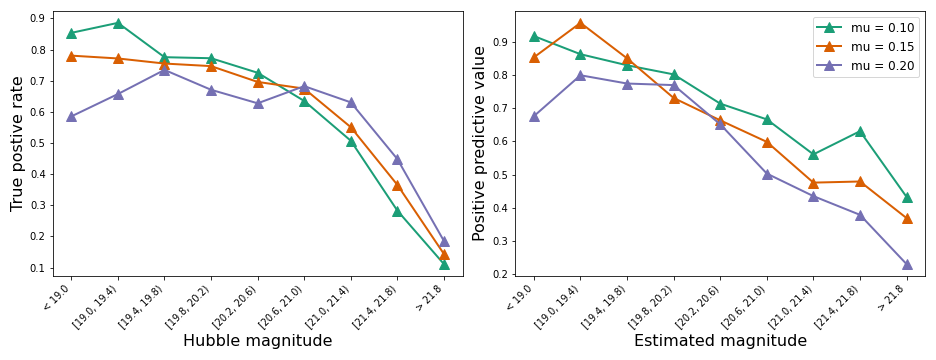
\includegraphics[width = \textwidth]{figures/prior_mu_sensitivty.png}
\end{subfigure}
\begin{subfigure}{\textwidth}
\begin{center}
\begin{tabular}{rrr}
\toprule
     mu &   TPR &   PPV \\
\midrule
 1000&  0.49 &  0.69 \\
 1500&  0.49 &  0.64 \\
 2000 &  0.52 &  0.49 \\
\bottomrule
\end{tabular}
\par\vspace{0pt}
\end{center}
\end{subfigure}\hfill
\caption{Sensitivity of summary statistics to Poisson mean parameter on number of stars. }
\end{figure}

\begin{figure}[ht]
\begin{subfigure}{\textwidth}
\centering
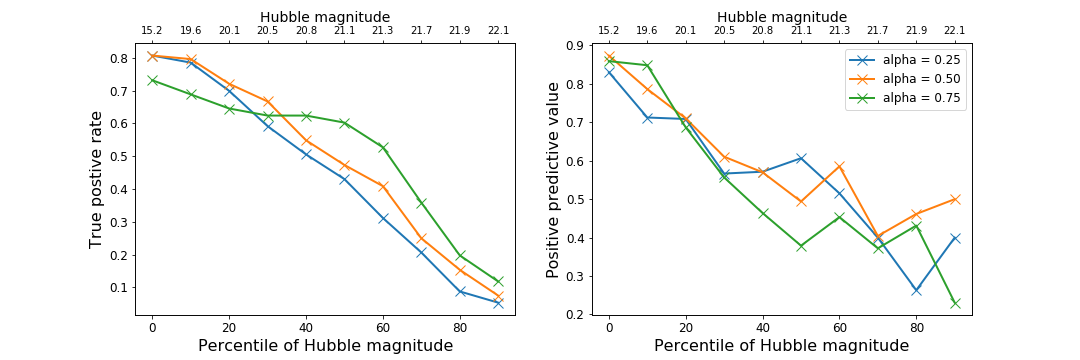
\includegraphics[width = \textwidth]{figures/prior_alpha_sensitivty.png}
\end{subfigure}
\begin{subfigure}{\textwidth}
\begin{center}
\begin{tabular}{rrr}
\toprule
 alpha &   TPR &   PPV \\
\midrule
  0.25 &  0.45 &  0.64 \\
  0.50 &  0.49 &  0.64 \\
  0.75 &  0.51 &  0.53 \\
\bottomrule
\end{tabular}
\par\vspace{0pt}
\end{center}
\end{subfigure}\hfill
\caption{Sensitivity of summary statistics to flux prior parameter $\alpha$. }
\end{figure}

\begin{figure}
    \centering
    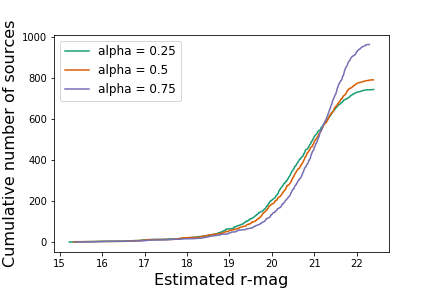
\includegraphics{figures/sensitivity_cdf_fluxes.png}
    \caption{Sensitivity of estimated flux distribution to flux prior parameter $\alpha$}
    \label{fig:cdf_sensitivity}
\end{figure}